\chapter{Erstellung des softaware/webdev-Docker-Containers}
\label{cha:implementation}
In diesem Abschnitt wird beschrieben, aus welchen Bestandteilen der Container besteht, warum diese Entscheidungen getroffen wurden und welche Probleme und Hürden sich bei der Entwicklung ergaben.
Weiters wird dargestellt, in welchen Aspekten der Container durch neue Kenntnisse beim Einsatz in echten Projekten weiterentwickelt wurde.

\section{Anwendungsszenarien}
Wie in \cref{cha:concept} erläutert, ist die grundlegende Idee des Containers, Node.js und npm oder yarn als versionierbare Abhängigkeit zu einem Projekt hinzuzufügen.
Anstatt der lokal Installation dieser Werkzeuge wird lediglich Docker auf dem System benötigt.
Folgend kann der Container wie in \cref{lst:docker-run-container} dargestellt gestartet werden.
\begin{lstlisting}[caption=Kommando zum Starten des softaware/webdev-Containers, language=bash, label=lst:docker-run-container]
docker container run -it --rm -v ${pwd}:/usr/src/app softaware/webdev:alpine-8.1.2
\end{lstlisting}
Das Kommando \verb|docker container run| entstammt der neuen Docker-CLI (seit Version 1.13 enthalten) und erzeugt einen Container auf Basis eines Image.
Die Parameter \verb|-it| erzeugen eine interaktive Shell zum Container.
Durch \verb|--rm| wird der Container nach dem Stoppen wieder entfernt.
Container sollten grundsätzlich keine Daten beinhalten, wodurch diese Option möglich wird und das System sauber hält.
Erst durch \verb|-v ${pwd}:/usr/src/app| können die Daten des Containers persistiert werden.
Dieses Kommando bindet das aktuelle Verzeichnis in das Arbeitsverzeichnis des Containers ein.
Dadurch können sowohl der Host, als auch der Container gleichzeitig mit diesem Verzeichnis arbeiten, wodurch es möglich wird, dass die Entwicklungsumgebung am Host läuft, npm allerdings im Container.
Am Ende des Kommandos wird das Docker-Image spezifiziert.
In diesem Fall wird die Alpine-Linux (vgl. \cref{sec:alpine-vs-debian}) mit der Node.js-Version 8.1.2 verwendet.
Das Ergebnis dieses Kommandos ist in \cref{fig:container-execution} zu sehen.
\begin{figure}[htbp]
    \centering
    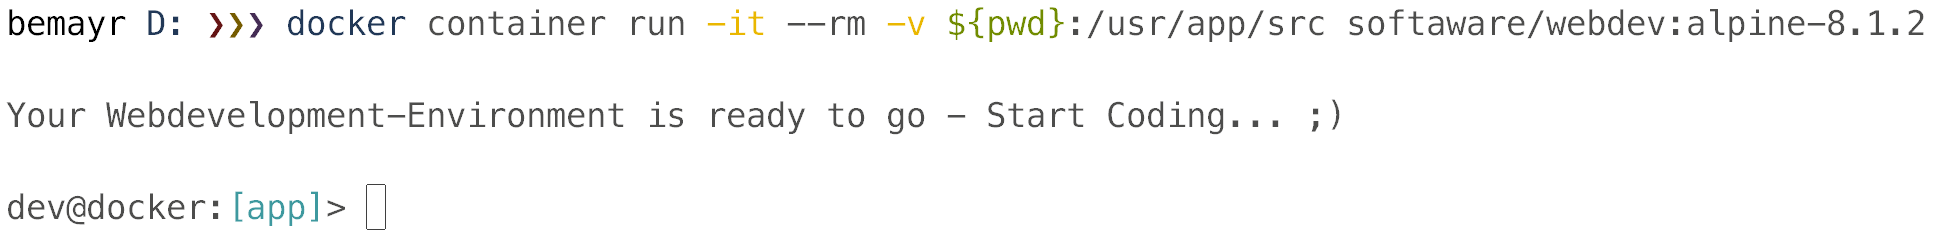
\includegraphics[width=0.95\linewidth,clip]{images/container-execution}
    \caption{Ausgabe beim Start des Containers}
\label{fig:container-execution}
\end{figure}

\subsubsection{Verwendungsmöglichkeiten des Containers}
Für den Container sind grundsätzlich die folgenden drei Anwendungsszenarien vorgesehen:

\begin{enumerate}
    \item Wie im vorangegangenen Beispiel gezeigt, kann mithilfe des Containers sehr schnell eine spezifische Kommandozeile mit installiertem Node.js und npm gestartet werden.
        Dies kann \zB zum Initialisieren eines Webprojektes mit \verb|npm init| verwendet werden.
    \item Weiters kann vom softaware/webdev-Image abgeleitet werden, um ein eigenes spezifischeres Image zu erstellen.
        In diesem können weitere Werkzeuge installiert werden, oder Ports des Containers explizit freigegeben werden. 
    \item Falls mithilfe der ersten Anwendungsweise ein Projekt erstellt wurde, wird empfohlen, danach das Startkommando mit derselben Containerversion als Skript zum Projekt hinzuzufügen.
        Dadurch kann die Entwickungsumgebung konistent reproduziert werden und als Abhängigkeit mit dem Projekt mitversioniert werden.
        Ein Beispiel dazu ist in \cref{sec:example} zu sehen.
\end{enumerate}
Im Folgenden wird das \emph{Dockerfile} erläutert, das die Basis des Containers darstellt und die eben beschriebenen Funktionen ermöglicht.

\section{Dockerfile}
\label{sec:dockerfile}
\lstinputlisting[caption=Alpine-Dockerfile,label={lst:dockerfile.alpine}]{listings/Dockerfile.alpine}

\subsubsection{Zeile 2}
Die \verb|FROM|-Anweisung ermöglicht es Docker-Images voneinander zu erben.
In diesem Fall wird vom offiziellen node-Image\footnote{\url{https://hub.docker.com/_/node/}} geerbt.
Dieses beinhaltet Node.js, npm und yarn, wodurch die gesamte Basisfunktionalität bereits vorhanden ist.

\verb|{{ node_version }}| ist keine Funktionalität von Docker, dies ist ein Platzhalter für die Versionsnummer des Node.js-Images im Build-Prozess (vgl. \cref{sec:build-process}).
Der Name des offiziellen Node.js-Images beginnt mit der Node.js-Versionsnummer und enthält die Art des Images als Suffix.
In diesem Fall wird von dem \emph{alpine}-Image abgeleitet und der Platzhalter im Build-Prozess durch die konkrete Versionsnummer ersetzt.

\subsubsection{Zeile 3}
Die früher verwendete \verb|MAINTAINER|-Anweisung in Dockerfiles wurde durch das flexiblere \verb|LABEL| ersetzt.
Durch den \emph{maintainer} werden Metadaten erstellt, die angeben wer für dieses Image verantwortlich ist, und an wen sich der Benutzer dessen wenden kann.

\subsubsection{Zeile 6}
Wie im Kommentar in Zeile 5 beschrieben, wird durch die \verb|ENV|-Anweisung die Umgebungsvariable \verb|PATH| erweitert.
Diese Änderung ermöglicht es, lokal installierte Node.js-Anwendungen als Kommandos zu verwenden.

In \cref{sec:global-package-installation} wurde bereits der Unterschied zwischen global und lokal installierten Anwendungen erläutert.
Im Container ist allerdings aufgrund der Isolierung das in \autocite{stackoverflow:nodemodules-hack:online} beschriebene Sicherheitsrisiko wesentlich geringer.
Anstatt der Erstellung eines eigenen Container-Images mit global installierten Paketen, sollten diese bei der Verwendung des Containers immer in der \emph{package.json}-Datei erfasst werden.
Dadurch muss kein eigenes Image gewartet werden und auch ohne dem Container sind alle Abhängigkeiten des Webprojektes definiert.

Diese Änderung an der Umgebungsvariable ist lediglich aus Kompatibilitätsgründen vorhanden, damit auch ältere Projekte, die sich historisch bedingt auf globale Abhängigkeiten verlassen, im Container verwendet werden können.
Die Konfiguration eines Webprojektes sollte allerdings nach \cref{subsub:packages-best-practice} erfolgen.

\subsubsection{Zeile 9}
Hier wird unter der Verwendung des Alpine-Linux-Paketmanagers \emph{apk} die Bourne Again Shell installiert.
Im Gegensatz zur Almquist Shell ist sie wesentlich weiter verbreitet und bietet erweiterte Funktionalität.
Durch den \verb|--no-cache| Parameter wird die Größe des fertigen Docker-Images möglichst klein gehalten.

\subsubsection{Zeile 12}
In Zeile 12 wird das aktuelle Arbeitsverzeichnis des resultierenden Containers auf \verb|/usr/src/app| gesetzt.
Die \verb|WORKDIR|-Anweisung eines Dockerfiles entpricht im wesentlich dem Wechsel in dieses Verzeichnis mit \verb|cd|.

\subsubsection {Zeile 15}
Das Aussehen der Eingabeaufforderung wird in Zeile 15 geändert.
Der Zweck dieser Änderung ist, dass der Entwickler auf den ersten Blick erkennen kann, ob er sich gerade im Containerm, oder außerhalb, befindet.
\lstinputlisting[caption=.bashrc (Bash-Konfigurationsdatei),label={lst:.bashrc},language=bash]{listings/.bashrc}
Durch das Dockerfile-Kommando \verb|COPY| wird die Datei \emph{.bashrc} in den Container kopiert.
Diese ist in \cref{lst:.bashrc} abgebildet.
Darin wird in Zeile 2 die Eingabeaufforderung durch das Setzen der Umgebungsvariable \verb|PS1| das Format \emph{dev@docker:[<aktuelles Verzeichnis>]>} zugewiesen.
Die kryptisch aussehende Notation ändert lediglich die Anzeigefarbe des aktuellen Verzeichnisses.
In Zeile 5 wird mit \verb|printf| eine Nachricht beim initialien Start des Containers ausgegeben.
Das Resultat ist in \cref{fig:container-execution} zu sehen.

\subsubsection {Zeile 16}
Beim Ausführen von Skripten, oder beispielsweise dem Deinstallieren von Paketen bietet npm auf der Kommandozeile die Möglichkeit der Autovervollständigung.
Diese wird aktiviert, indem das Kommando \verb|npm completion| ein Shell-Skript erstellt, das an die benutzerspezifische Shell-Konfiguration angehängt wird.

Das Ergebnis von \verb|npm completion| war in einer früheren Version des Containers bereits in \emph{.bashrc} integriert.
Falls dieses allerdings bei unterschiedlichen npm-Versionen unterschiedlich ausfällt, würde die Autovervollständigung nicht korrekt funktionieren.
Durch das nachträgliche Hinzufügen des Ergebnisses mithilfe der \verb|RUN|-Anweisung ist nun sichergestellt, dass das Ergebnis von \verb|npm completion| immer zur verwendeten npm-Version passt.

\subsubsection {Zeile 17}
In Zeile 17 wird das standardmäßige Startkommando des Containers auf die Bourne Again Shell festgelegt.
Der verwendete Node.js-Container startet standardmäßig mit dem Kommando \verb|node| ohne weitere Parameter.
Da der softaware/webdev-Container allerdings zur interaktiven Entwicklung gedacht ist, wird dieses Standardverhalten überschrieben.
In \cref{sub:examples} wird gezeigt, dass dieses Kommando beim Ausführen des Containers überschreiben lässt, wodurch sich der Container auch zum Skripten eignet.

In einer früheren Version des Containers wurde beim Start ein Skript aufgerufen, das überprüft ob das aktuelle Verzeichnis ein Webprojekt ist.
In diesem Fall wurde \verb|npm install| aufgerufen, um alle Abhängigkeiten zu überprüfen und im Fall von fehlenden Paketen, diese nachzuinstallieren.
Da dieses Verhalten für den Verwender unerwartet ist, allerdings bei jedem Start einige Sekunden kostet, wurde dieses Feature wieder entfernt. 


\section{Build-Prozess}
\label{sec:build-process}

https://docs.docker.com/docker-hub/github/
Namenskonenvtion

\lstinputlisting[caption=\emph{create-image.ps1} (Build-Skript des Containers),label={lst:create-image.ps1}]{listings/create-image.ps1}

\begin{figure}[htbp]
    \centering
    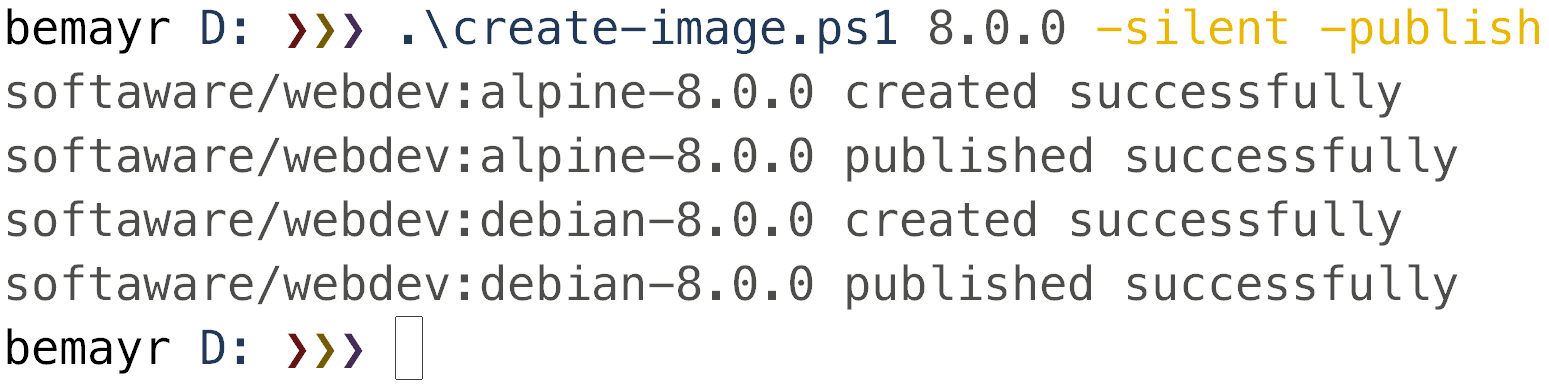
\includegraphics[width=0.75\linewidth,clip]{images/create-image}
    \caption{Ausgabe des Build-Prozesses für Node.js 8.0}
\label{fig:create-image}
\end{figure}

\section{Alpine-Linux vs. Debian}
\label{sec:alpine-vs-debian}
\lstinputlisting[caption=Debian-Dockerfile,label={lst:dockerfile.debian}]{listings/Dockerfile.debian}

\section{Dokumentation}
\label{sec:documentation}

\subsubsection{GitHub}
\label{sub:github}
\subsubsection{Docker Hub}
\label{sub:dockerhub}
Der Container ist im Docker Hub\footnote{\url[]} veröffentlicht
\subsubsection{Microbadger}
\label{sub:microbadger}


\section{Beispielanwendung des Containers}
\label{sec:example}
\lstinputlisting[caption=docker-webdev.ps1 (Container-Start-Skript),label={lst:docker-webdev.ps1}]{listings/docker-webdev.ps1}

\begin{figure}[htbp]
    \centering
    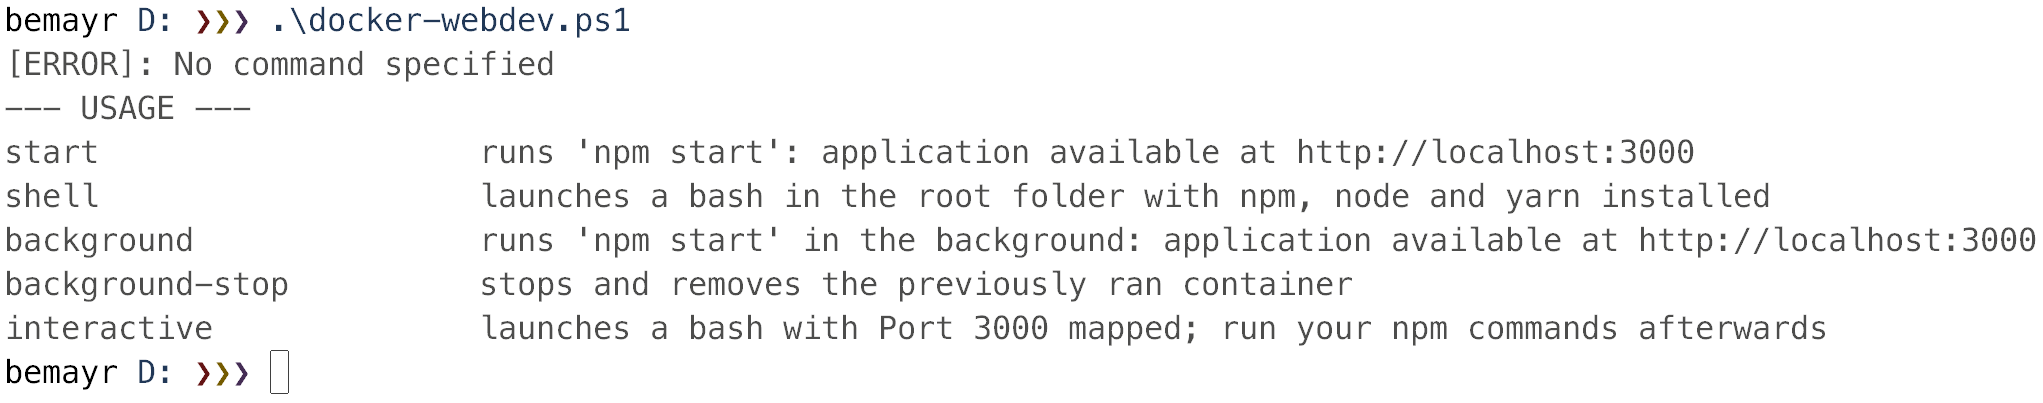
\includegraphics[width=0.95\linewidth,clip]{images/docker-webdev}
    \caption{Hilfe zum Startskript des Containers in einer echten Applikation}
\label{fig:docker-webdev}
\end{figure}


\section{Probleme und Besonderheiten}
\label{sec:container-problems}

\begin{description}
    \item[Kendo UI Sass Build]
    \item[different OSs]
    \item[prevent IDE automatic install]
    \item[File Detection]
    \item[Typescript node modules]
    \item[Port-mapped application containers]
    \item[optional]
\end{description}
